\chapter{MARP Results with QRAcc}

In this chapter, we present the benefits of using MARP on QRAcc, our hybrid AIMC accelerator architecture. MARP can achieve a 26.19\% reduction in energy consumption and a 19.65\% reduction in latency on MobileNetV2 inference in QRAcc.  

\label{chap:marp_qracc}

\section{Extracting Statistics from QRAcc}

We compile and perform inference on the MLPerfTiny models using MARP, while at the same time tracking statistics in a global data structure. QRAcc's individual RTL blocks fill up the statistics data structure during behavioral simulation. Every new layer, the statistics data structure is exported into a CSV row and then cleared for the next layer. The statistics data structure contains the following fields:

\begin{enumerate}
    \item \texttt{statActmem...}: Counts read and write operations to the Activation Memory, distinguishing between internal and external port access.
    \item \texttt{statFL...}: Counts read and write operations to the Free List memory.
    \item \texttt{statSeqAcc...}: Tracks operations related to the Sequential Accumulator, including weight writes, total operations, and the number of Multiply-Accumulate (MAC) operations.
    \item \texttt{statWQ...}: Counts read and write operations to the Weight Queue.
    \item \texttt{cyclesIdle}: Number of cycles the accelerator was idle.
    \item \texttt{cyclesLoad...}: Cycles spent on loading data, such as activations, scalers, biases, and weights for both analog and digital units.
    \item \texttt{cyclesCompute...}: Cycles spent on computation, separated into analog and digital processing phases.
    \item \texttt{cyclesReadActivation}: Cycles consumed while reading out the resulting activations from the memory.
\end{enumerate}

Given the characterizations on QRAcc in Chapter \ref{chap:qracc} and the tracked statistics, we calculate the energy consumption of QRAcc. For most of the state-dependent energy components, 

\begin{equation}
    E_{state} = P_{qracc,state}\cdot N_{cycles,state}\cdot T_{clk}
\end{equation}

where $T_{clk}$ is 50MHz. For the "Load Weights" state in particular, we use the following equation:
\begin{equation}
    E_{load\_weights} = N_{cycles,load\_weights}\cdot T_{clk}(32\cdot P_{seqacc,write,bit}\cdot P_{qracc,load\_weights})
\end{equation}

where $P_{seqacc,write,per-bit}$ is power consumed by writing a single bit to SeqAcc as measured in Chapter \ref{chap:qracc}. SeqAcc writes 32 bits per cycle, so we multiply by 32. $P_{qracc,load\_weights}$ is the power consumed by the QRAcc architecture when loading weights, which was measured in Chapter \ref{chap:qracc}.

Lastly, for the "Compute Analog" state, we use the following equation:
\begin{equation}
    E_{analog} = N_{cycles,analog}\cdot T_{clk}(K\cdot P_{seqacc,mac,column}\cdot P_{qracc,analog})
\end{equation}

where $K$ is the number of output channels of the layer being computed, and the rest are values we measured in Chapter \ref{chap:qracc}. We scale the power by $K$ because SeqAcc only activates $K$ columns when only $K$ output channels are computed. 

\section{Latency Results}

\begin{figure}[htbp]
    \centering
    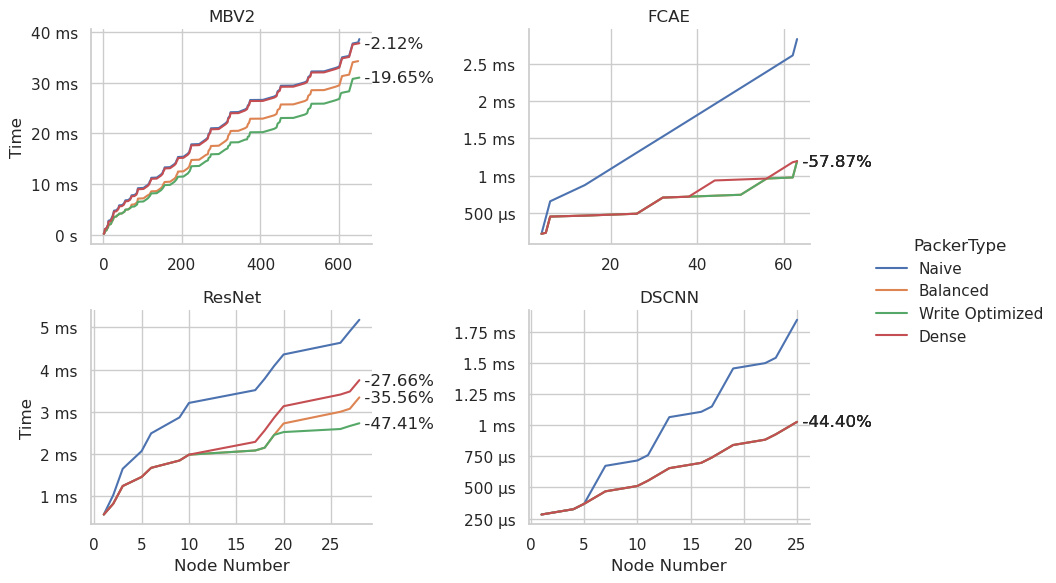
\includegraphics[width=\textwidth]{images/marp_qracc/timeline.png}
    \caption{Line plot of the total inference time vs node being processed in QRAcc for inference in each of the 4 MLPerfTiny models. At the end of the lines, we annotate the reduction in inference time vs the naive single-mapping packer.}
    \label{fig:timeline}
\end{figure}

\begin{figure}[htbp]
    \centering
    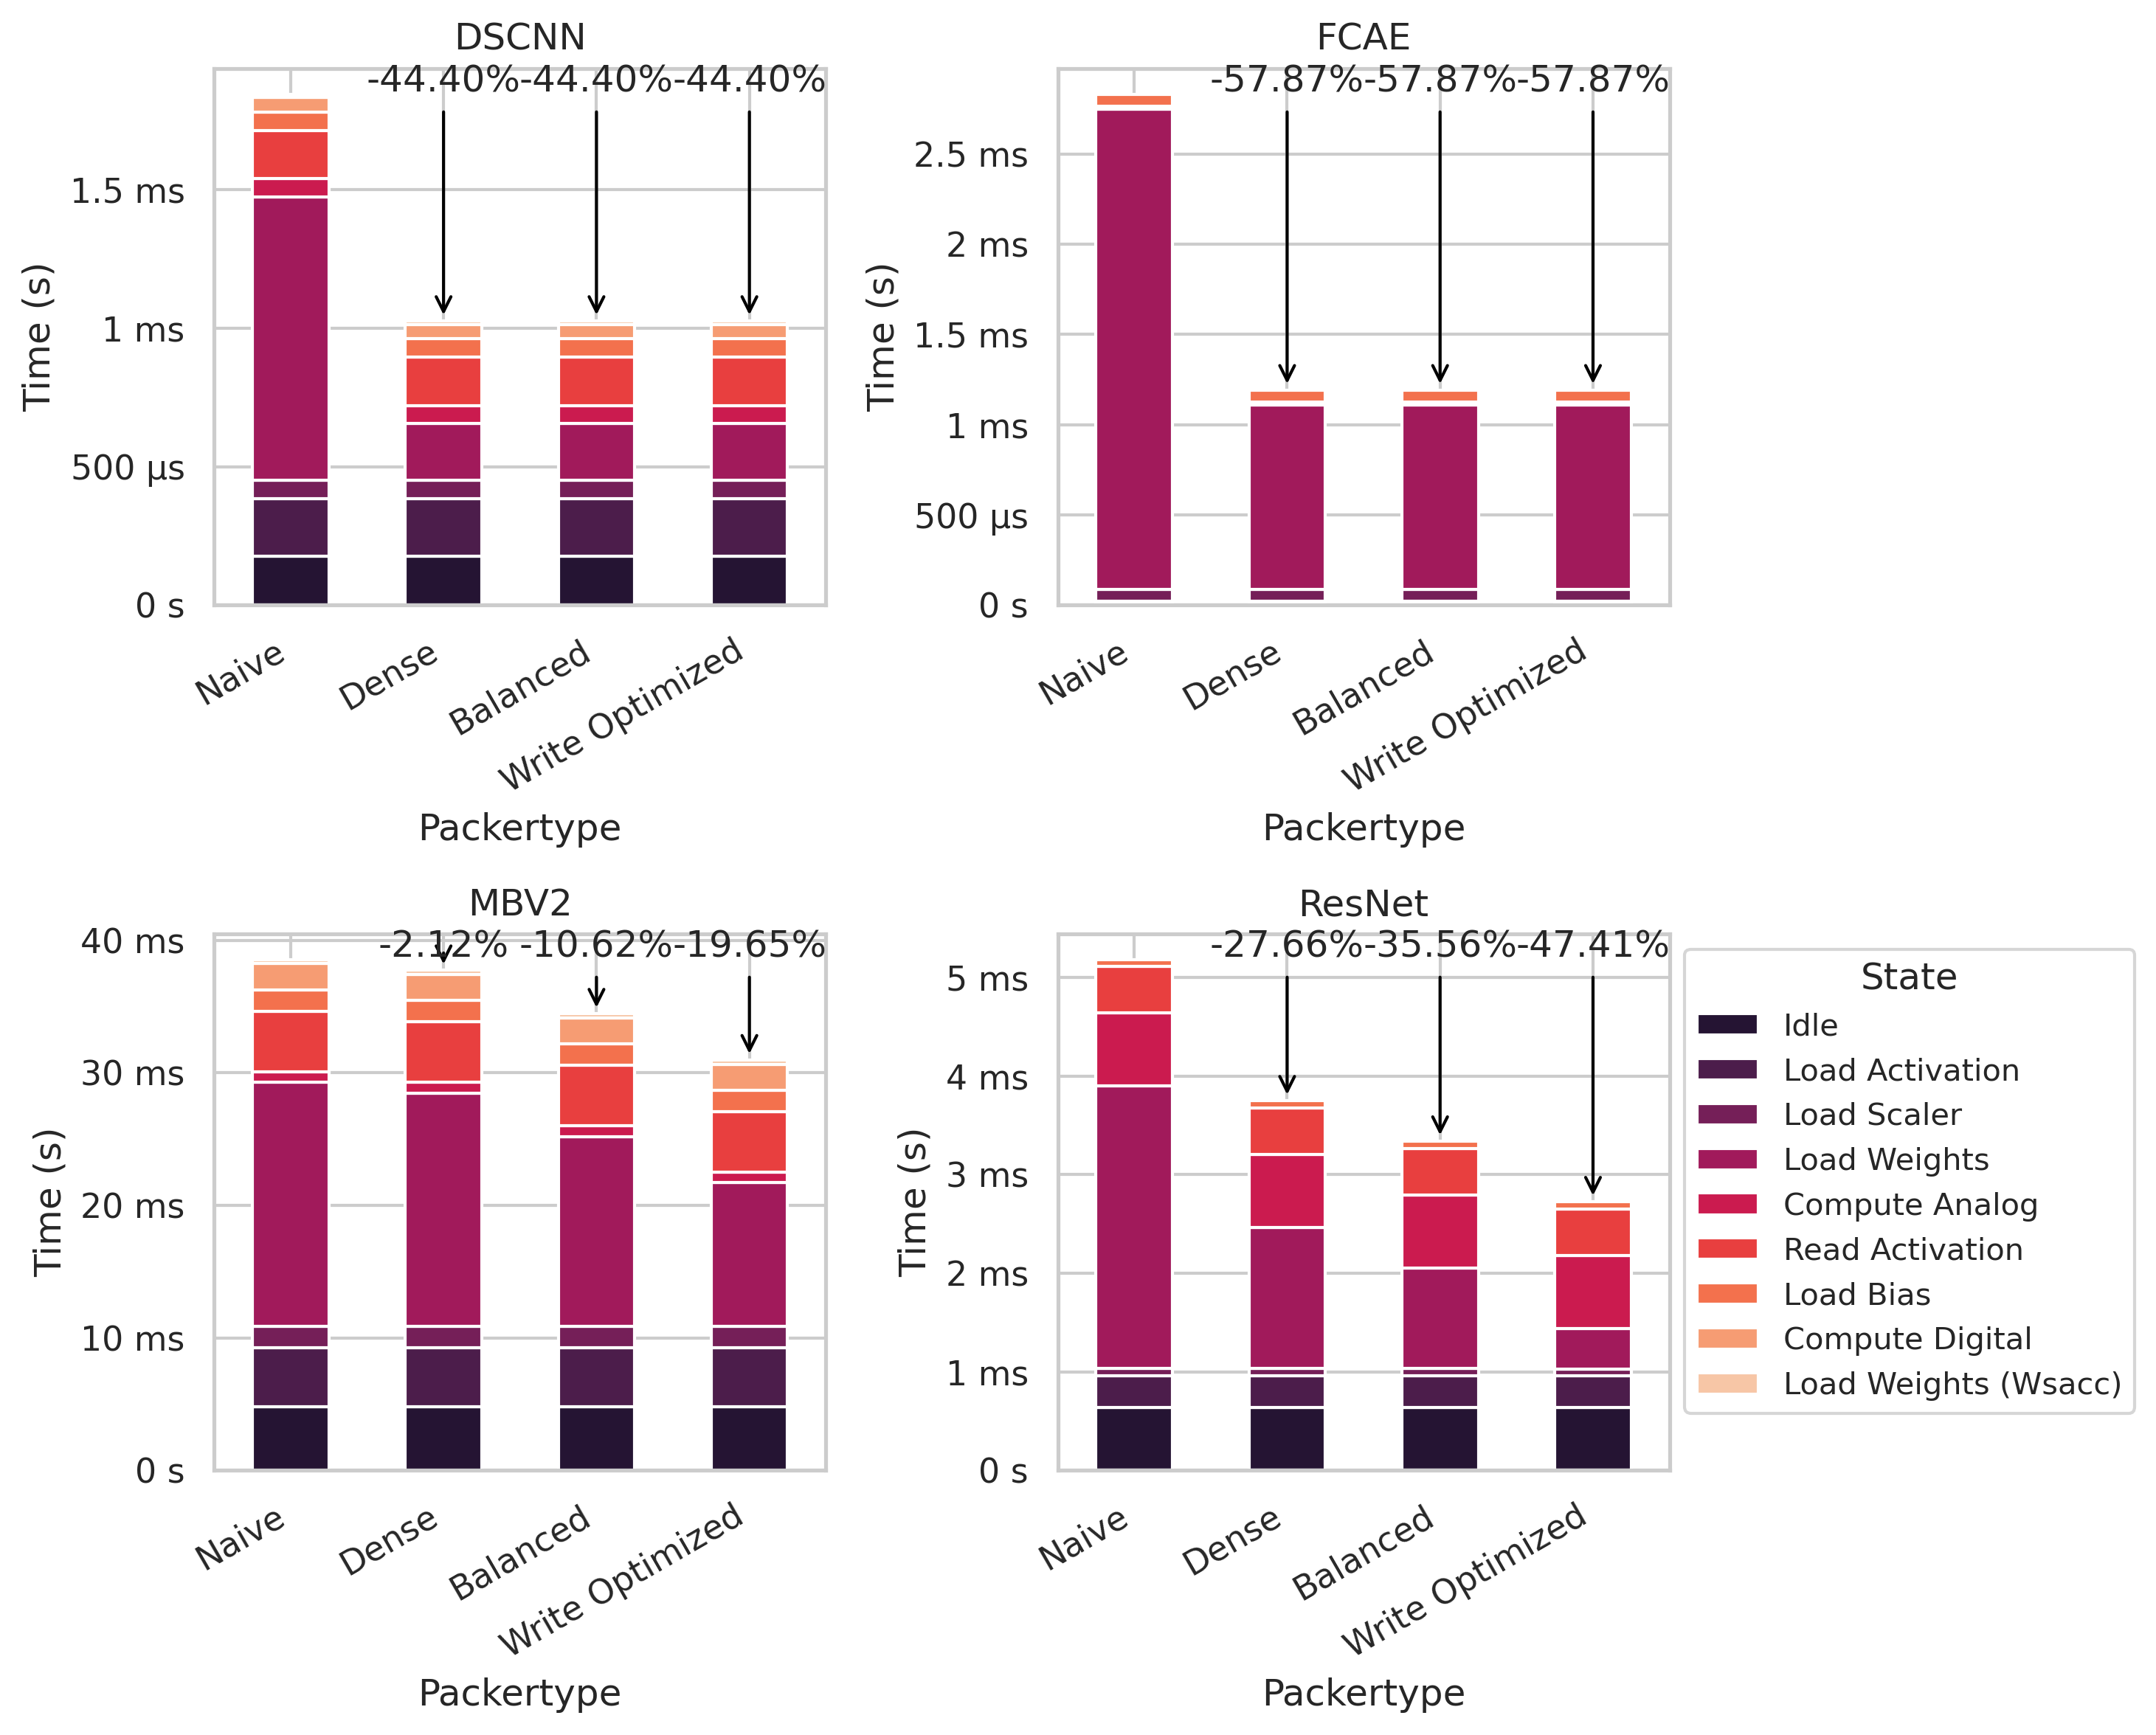
\includegraphics[width=\textwidth]{images/marp_qracc/time_bars.png}
    \caption{Stacked bar chart of the time spent in each state of QRAcc for inference in each of the 4 MLPerfTiny models}
    \label{fig:time_bars}
\end{figure}

Figure \ref{fig:timeline} shows the total inference time vs node being processed in QRAcc for inference in each of the 4 MLPerfTiny models. The lines show the total inference time for each node, and at the end of the lines, we annotate the reduction in inference time vs the naive single-mapping packer. We see that of the packers, the naive packer tends to take the longest inference time, then the balanced packer, then the write-optimized packer.

The main cause of the reduction in inference time can be seen by taking a look at Figure \ref{fig:time_bars}, which shows a stacked bar chart of the time spent in each state of QRAcc for inference in each of the 4 MLPerfTiny models. For all of the models' naive single-mapping, the "Load Weights" state takes the longest due to the large number of writes to the SeqAcc memory array. As the packer used optimizes for less writes, the "Load Weights" state takes less time and this is reflected in the total inference time. 

For the FC-AE and DS-CNN models, they tend to have much a higher number of smaller matrices than the other models. Hence, the latency reductions on these models are massive at -44.4\% and -57.85\%. However, MARP on these models retains the same number of bins for all 4 packers, so the reduction in inference time is the same for all the packings. Interestingly, the time spent loading weights dominates in FC-AE inference. We attribute this to the fact that FC-AE is a model made up of mostly fully-connected layers, which turn into simple matrix multiplications. This is equivalent to a pointwise convolution with a 1x1 image with 640 input channels and 640 output channels. Since there is only one pixel to process, the computation time is extremely short compared to the time spent loading weights.

For the MobileNetV2 model, we see more distinction in the different packers. On MobileNetV2, despite the dense packer being able to reduce the bins from 91 to 34, the dense packing has such a random access pattern that the number of writes is essentially the same as the naive single-mapping packer leading to a very low reduction in inference time of -2.12\%. On the other hand the balanced and write-optimized packers are able to reduce the number of writes instead of just the number of bins, leading to a reduction in inference time of -10.62\% and -19.65\% respectively.

For the ResNet model, we see that even the dense packer is able to reduce the inference time by as much as -27.66\% which we attribute to the sheer amount of utilization gained. From 15 bins, all of the packers of the ResNet model are able to reduce the number of bins to 2, which leads to a significant reduction in the number of writes to the SeqAcc memory array. The balanced packer and write-optimized packer are further able to make sure to use the same bin for consecutive layers, which leads to a further reduction in inference time of -35.56\% and -47.41\% respectively.

\section{Energy Results}

\begin{figure}[htbp]
    \centering
    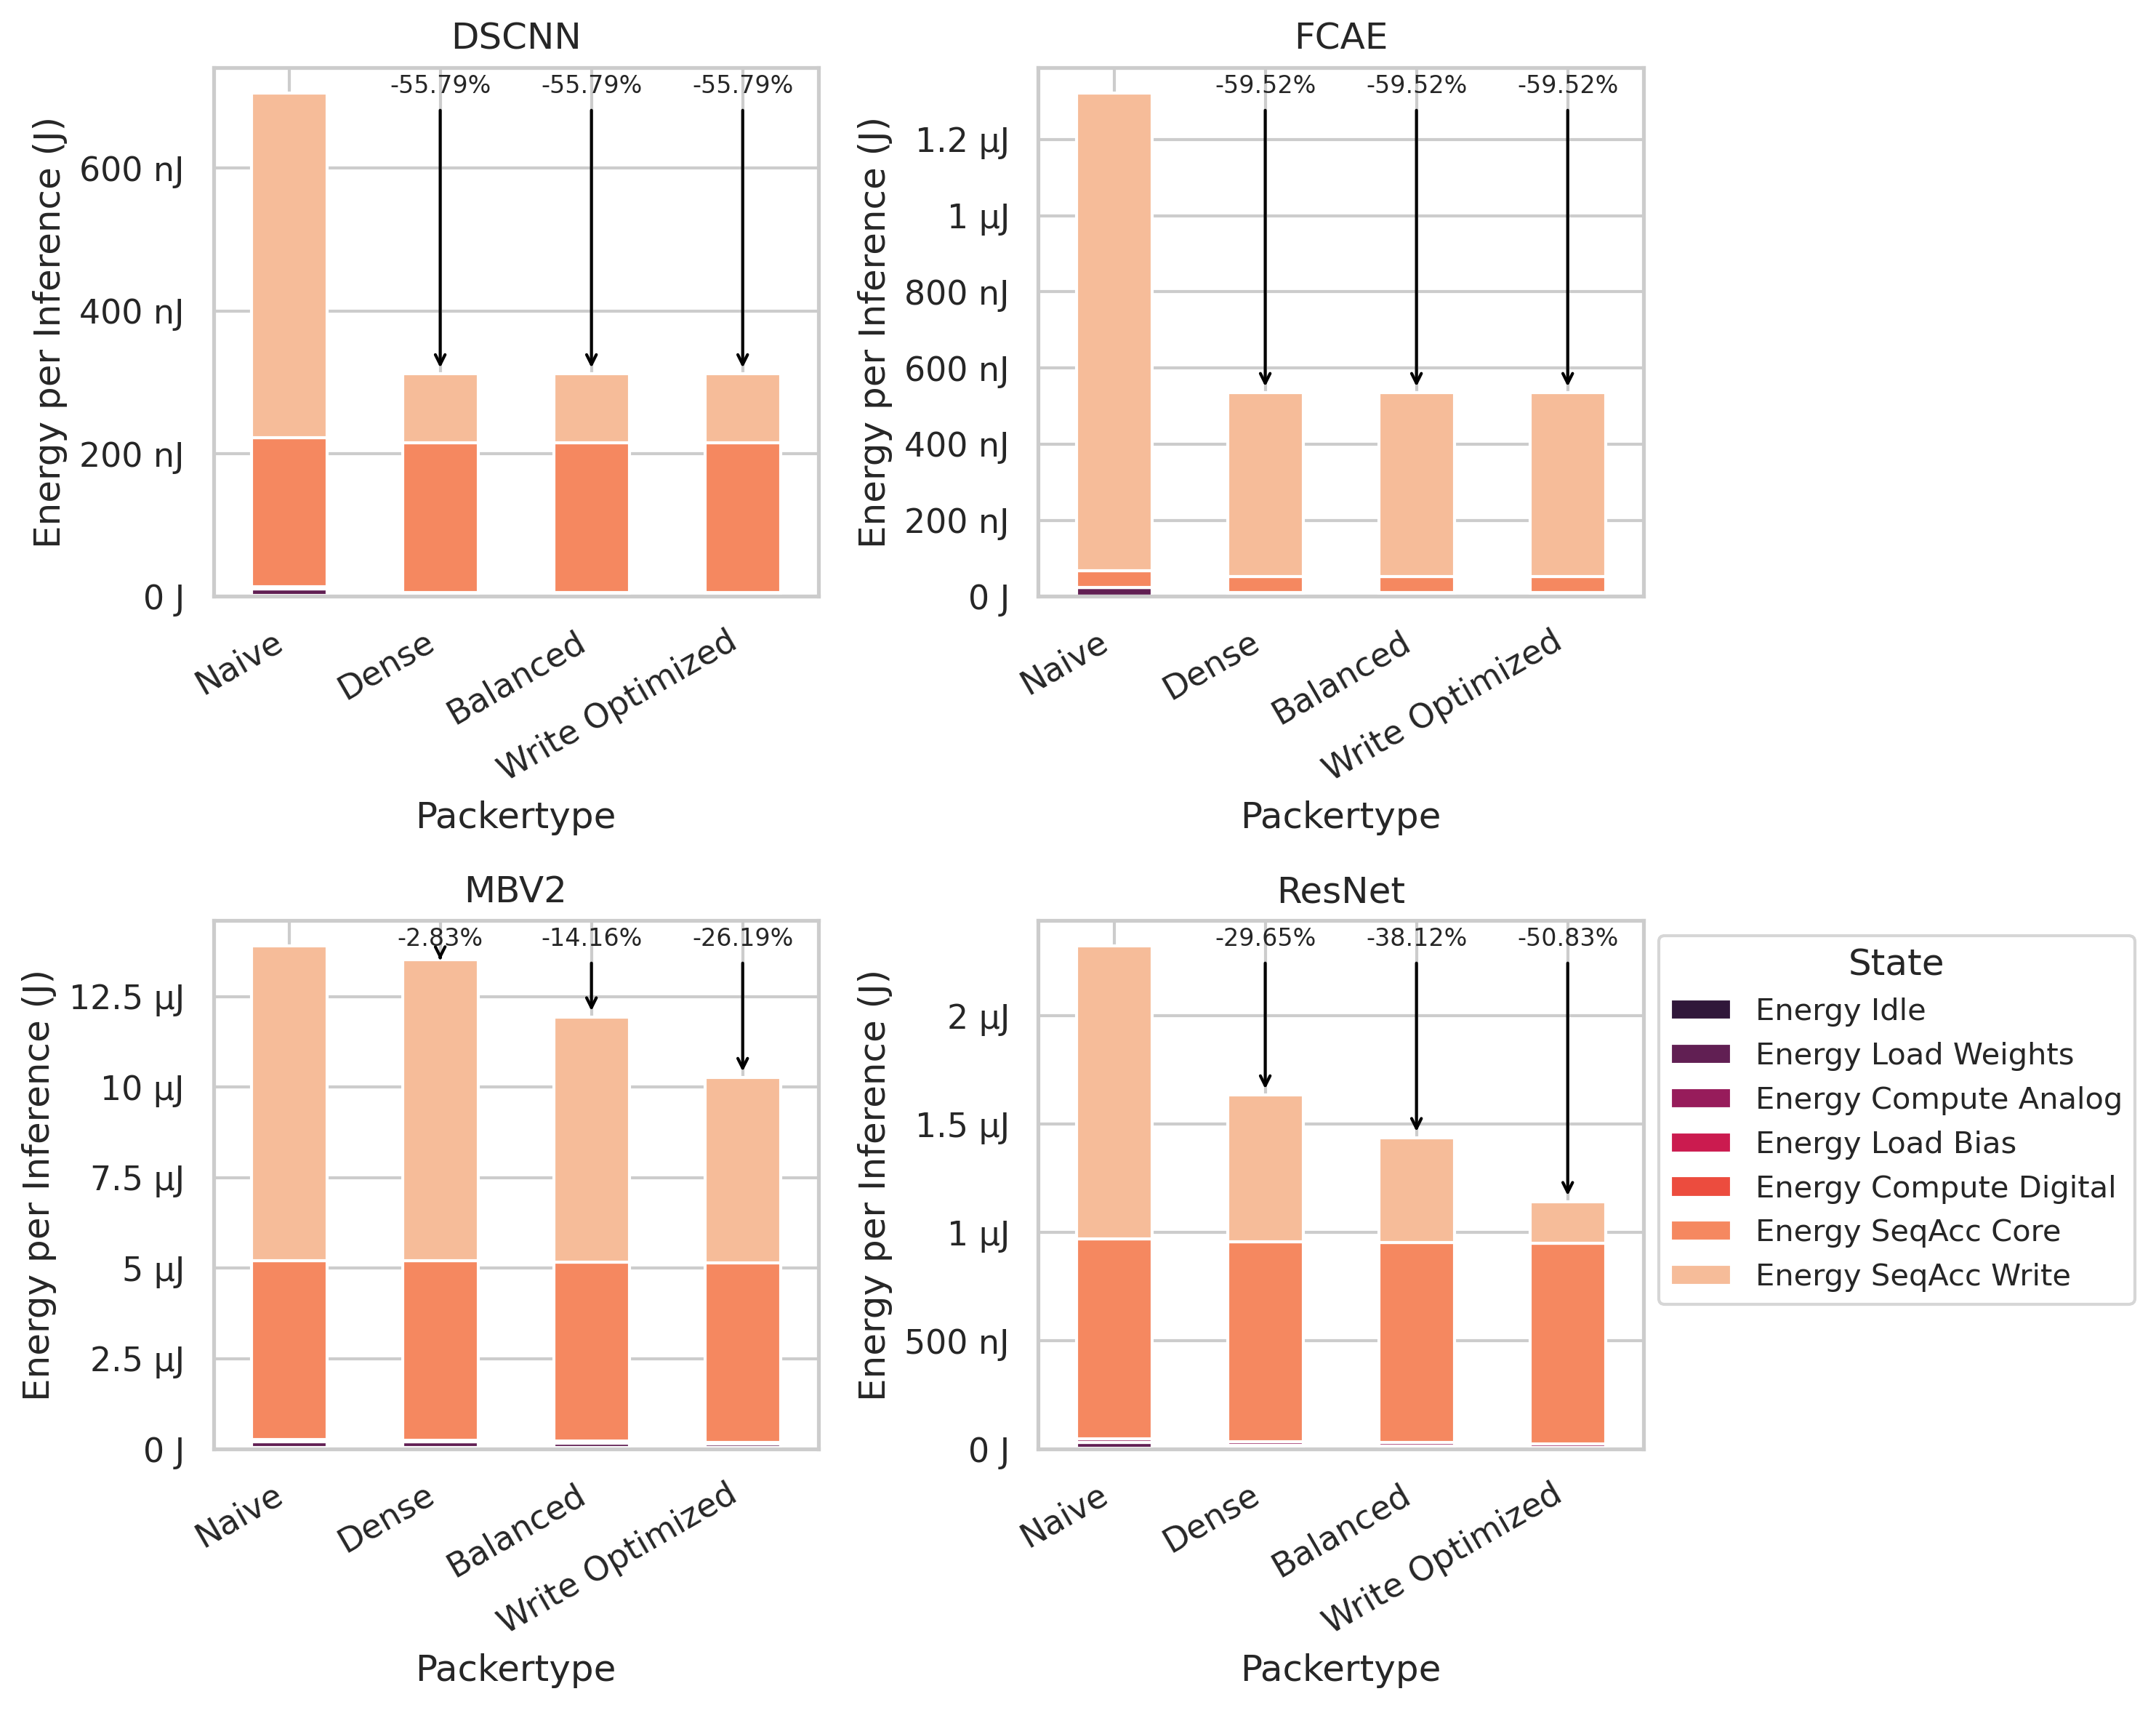
\includegraphics[width=\textwidth]{images/marp_qracc/energy_bars.png}
    \caption{Stacked bar chart of the energy used for inference in each of the 4 MLPerfTiny models}
    \label{fig:energy_bars}
\end{figure}

\begin{figure}[htbp]
    \centering
    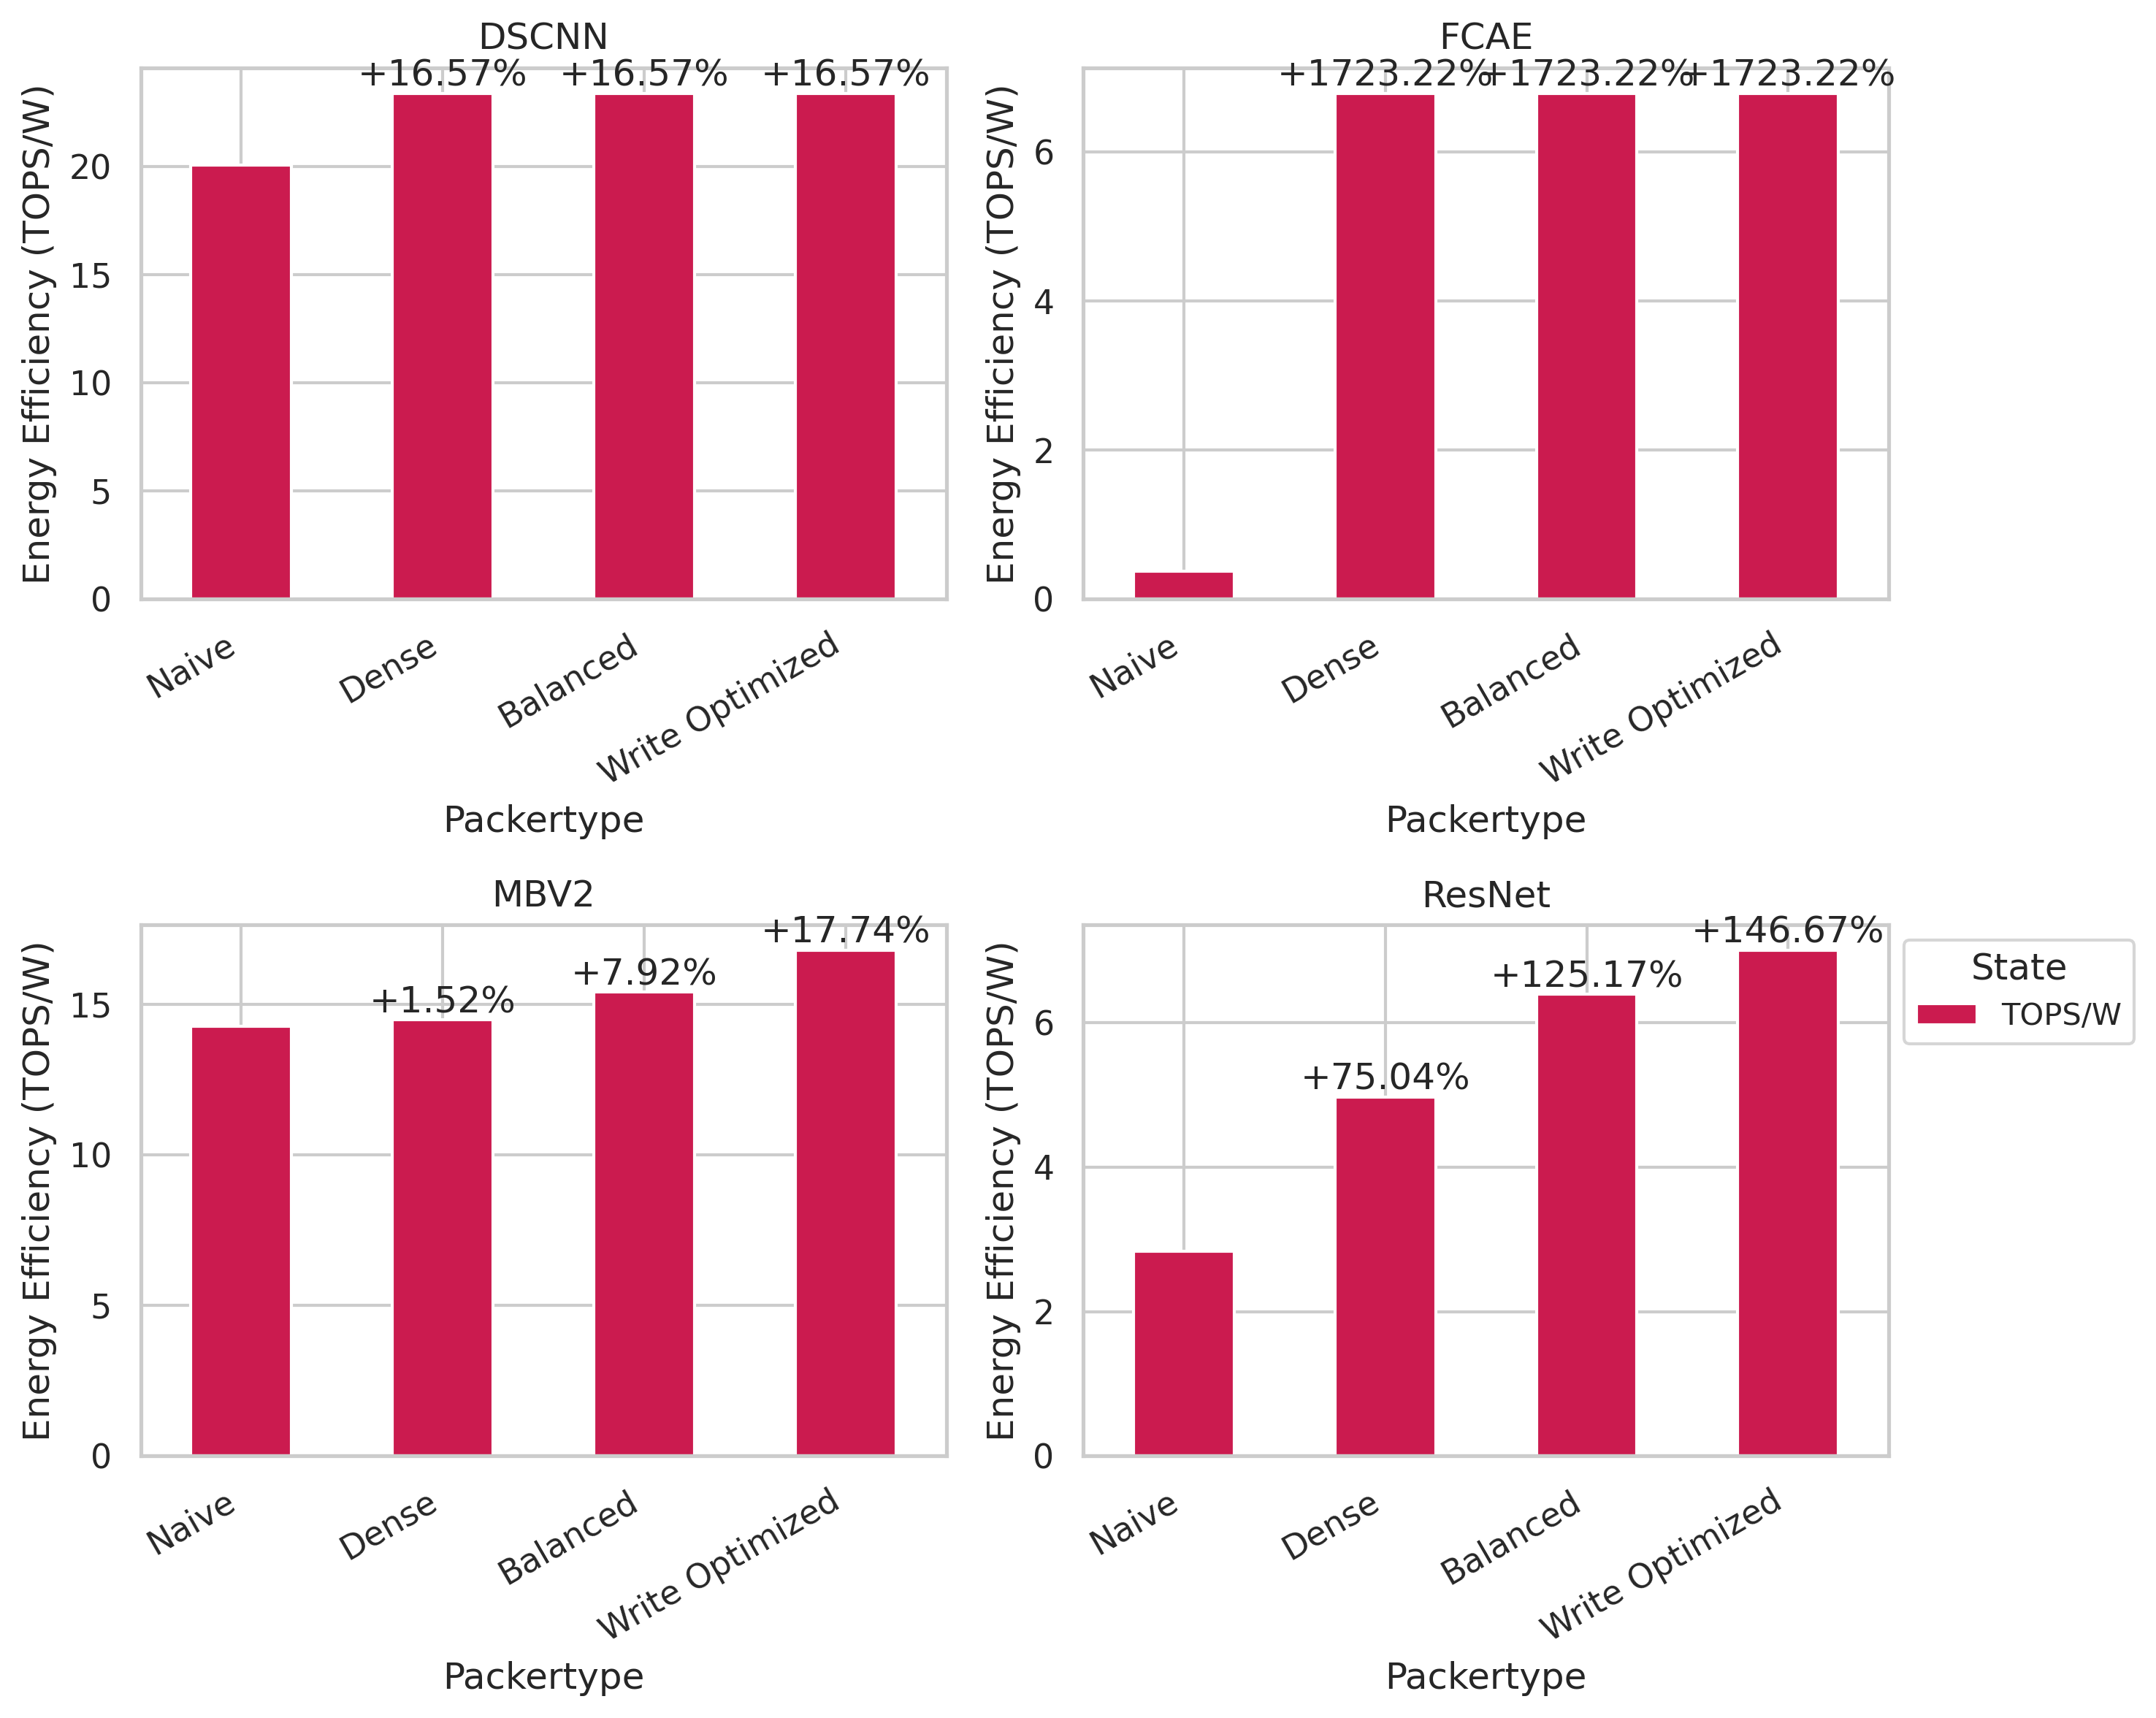
\includegraphics[width=\textwidth]{images/marp_qracc/tops_bars.png}
    \caption{Stacked bar chart of the energy efficiency (TOPS/W) of QRAcc for inference in each of the 4 MLPerfTiny models}
    \label{fig:tops_bars}
\end{figure}

Figure \ref{fig:energy_bars} shows a stacked bar chart of the energy used for inference in each of the 4 MLPerfTiny models. We see that for all the models, the naive single-mapping packer uses the most energy per inference, followed by the dense packer, then the balanced packer, and finally the write-optimized packer. The main reason for the energy savings is the same as the latency savings: the reduction in the number of writes to the SeqAcc memory array. By skipping the load weights state whenever the previously loaded bin into QRAcc is the bin of the current layer, we can save on all of the write energy.

The FC-AE and DS-CNN models show the most energy savings as with the latency results. MARP reduced the FC-AE and DS-CNN energy consumptions by -55.79\% and -59.52\% respectively. This is a higher gain than the latency results because the energy consumed by the "Load Weights" state is higher than the latency added by it. Again, for the different packers, MARP obtains no significant difference in energy savings owing to the fact that packing allows the use of very few bins (1 for FC-AE and 2 for DS-CNN).

For the MobileNetV2 model, we see that the dense packer is able to reduce the energy consumption by only -2.83\% compared to the naive single-mapping packer. However, the balanced and write-optimized packers are able to reduce the energy consumption by -14.16\% and -26.19\% respectively. There are lower reductions in energy consumption for MobileNetV2 due to its massive layer matrix sizes, as there are still many writes to the SeqAcc memory array even with packings. Not only that, but a significant number of the layers in MobileNetV2 are depthwise convolutions, which are mapped to the digital core of QRAcc. This portion of the energy consumption is not reduced by MARP, as MARP only optimizes the AIMC core of QRAcc.

Lastly, for the ResNet model, we see that the dense packer is able to reduce the energy consumption by -29.65\% compared to the naive single-mapping packer. The balanced packer and write-optimized packer are able to reduce the energy consumption by -38.12\% and -50.83\% respectively. The ResNet model has a very high number of layers and unlike MobileNetV2, it does not have depthwise convolutions. This means that the majority of the layers are mapped to the SeqAcc memory array, which allows MARP to reduce the number of writes to the SeqAcc memory array significantly. However, we still see the benefits of the write-optimized packer due to the number of bins (16) needed for the ResNet model. Having a higher number of bins means that there is a higher chance that the next layer will not be in the same bin as the previous layer, which the write-optimized packer is able to optimize for.

Figure \ref{fig:tops_bars} shows a stacked bar chart of the energy efficiency (TOPS/W) of QRAcc for inference in each of the 4 MLPerfTiny models. Note that this energy efficiency is expected to be lower than that reported in Chapter \ref{chap:qracc} because the energy efficiency reported in Chapter \ref{chap:qracc} is the peak energy efficiency of QRAcc, while this is the energy efficiency of practical inference, accounting for the energy consumed while moving data into QRAcc as well.

We see MARP allows the energy efficiency for all the models go to at least around 5 TOPS/W or above, which is relatively efficient even including the energy consumption of data movement. While these energy efficiency values are lower than what would usually be expected, it is high if you consider that these are system-level measurements. In existing literature, most of the high energy efficiency values are reported on the bank level (for AIMCs) and L2-array level (for digital accelerators). 

These levels of energy efficiency can enable the use of QRAcc in edge AI applications, which was the main goal of this work. 

\section{Influence of Layer Type}

We further analyze the influence of layer type such as depthwise, input feature map sizes, kernel sizes, and node order on the performance. Figure \ref{fig:duration_tops_scatter} shows a scatter plot of the latency vs energy of different layers in the MLPerfTiny models. The sizes of the markers in the scatter plot represent the size of the input feature map of the layer, while the colors represent the size of the kernel. Cross-marks are depthwise convolutions, while circles are regular convolutions and matrix multiplications.

We see that layers with larger input feature maps tend to take longer (but not always) to process, which is expected as larger input feature maps require more computations. However, we also see that they can also obtain very high energy efficiencies when MARP packs then with high emphasis on the write optimization. 

We also see that depthwise convolutions tend to take much faster to process than regular convolutions and matrix multiplications. This is as expected, as they are composed of much fewer MACs and operations than regular convolutions and matrix multiplications. However, we can also see that the energy efficiencies of calculating them are around the same as that of the regular convolutions and matrix multiplications. With the naive and dense packers, the energy efficiency of depthwise convolutions is sometimes higher than that of regular convolutions and matrix multiplications. However, as we optimize for writing in the AIMC array less, the energy efficiency of most of the regular convolutions are now competitive with the depthwise convolutions.

\begin{figure}[htbp]
    \centering
    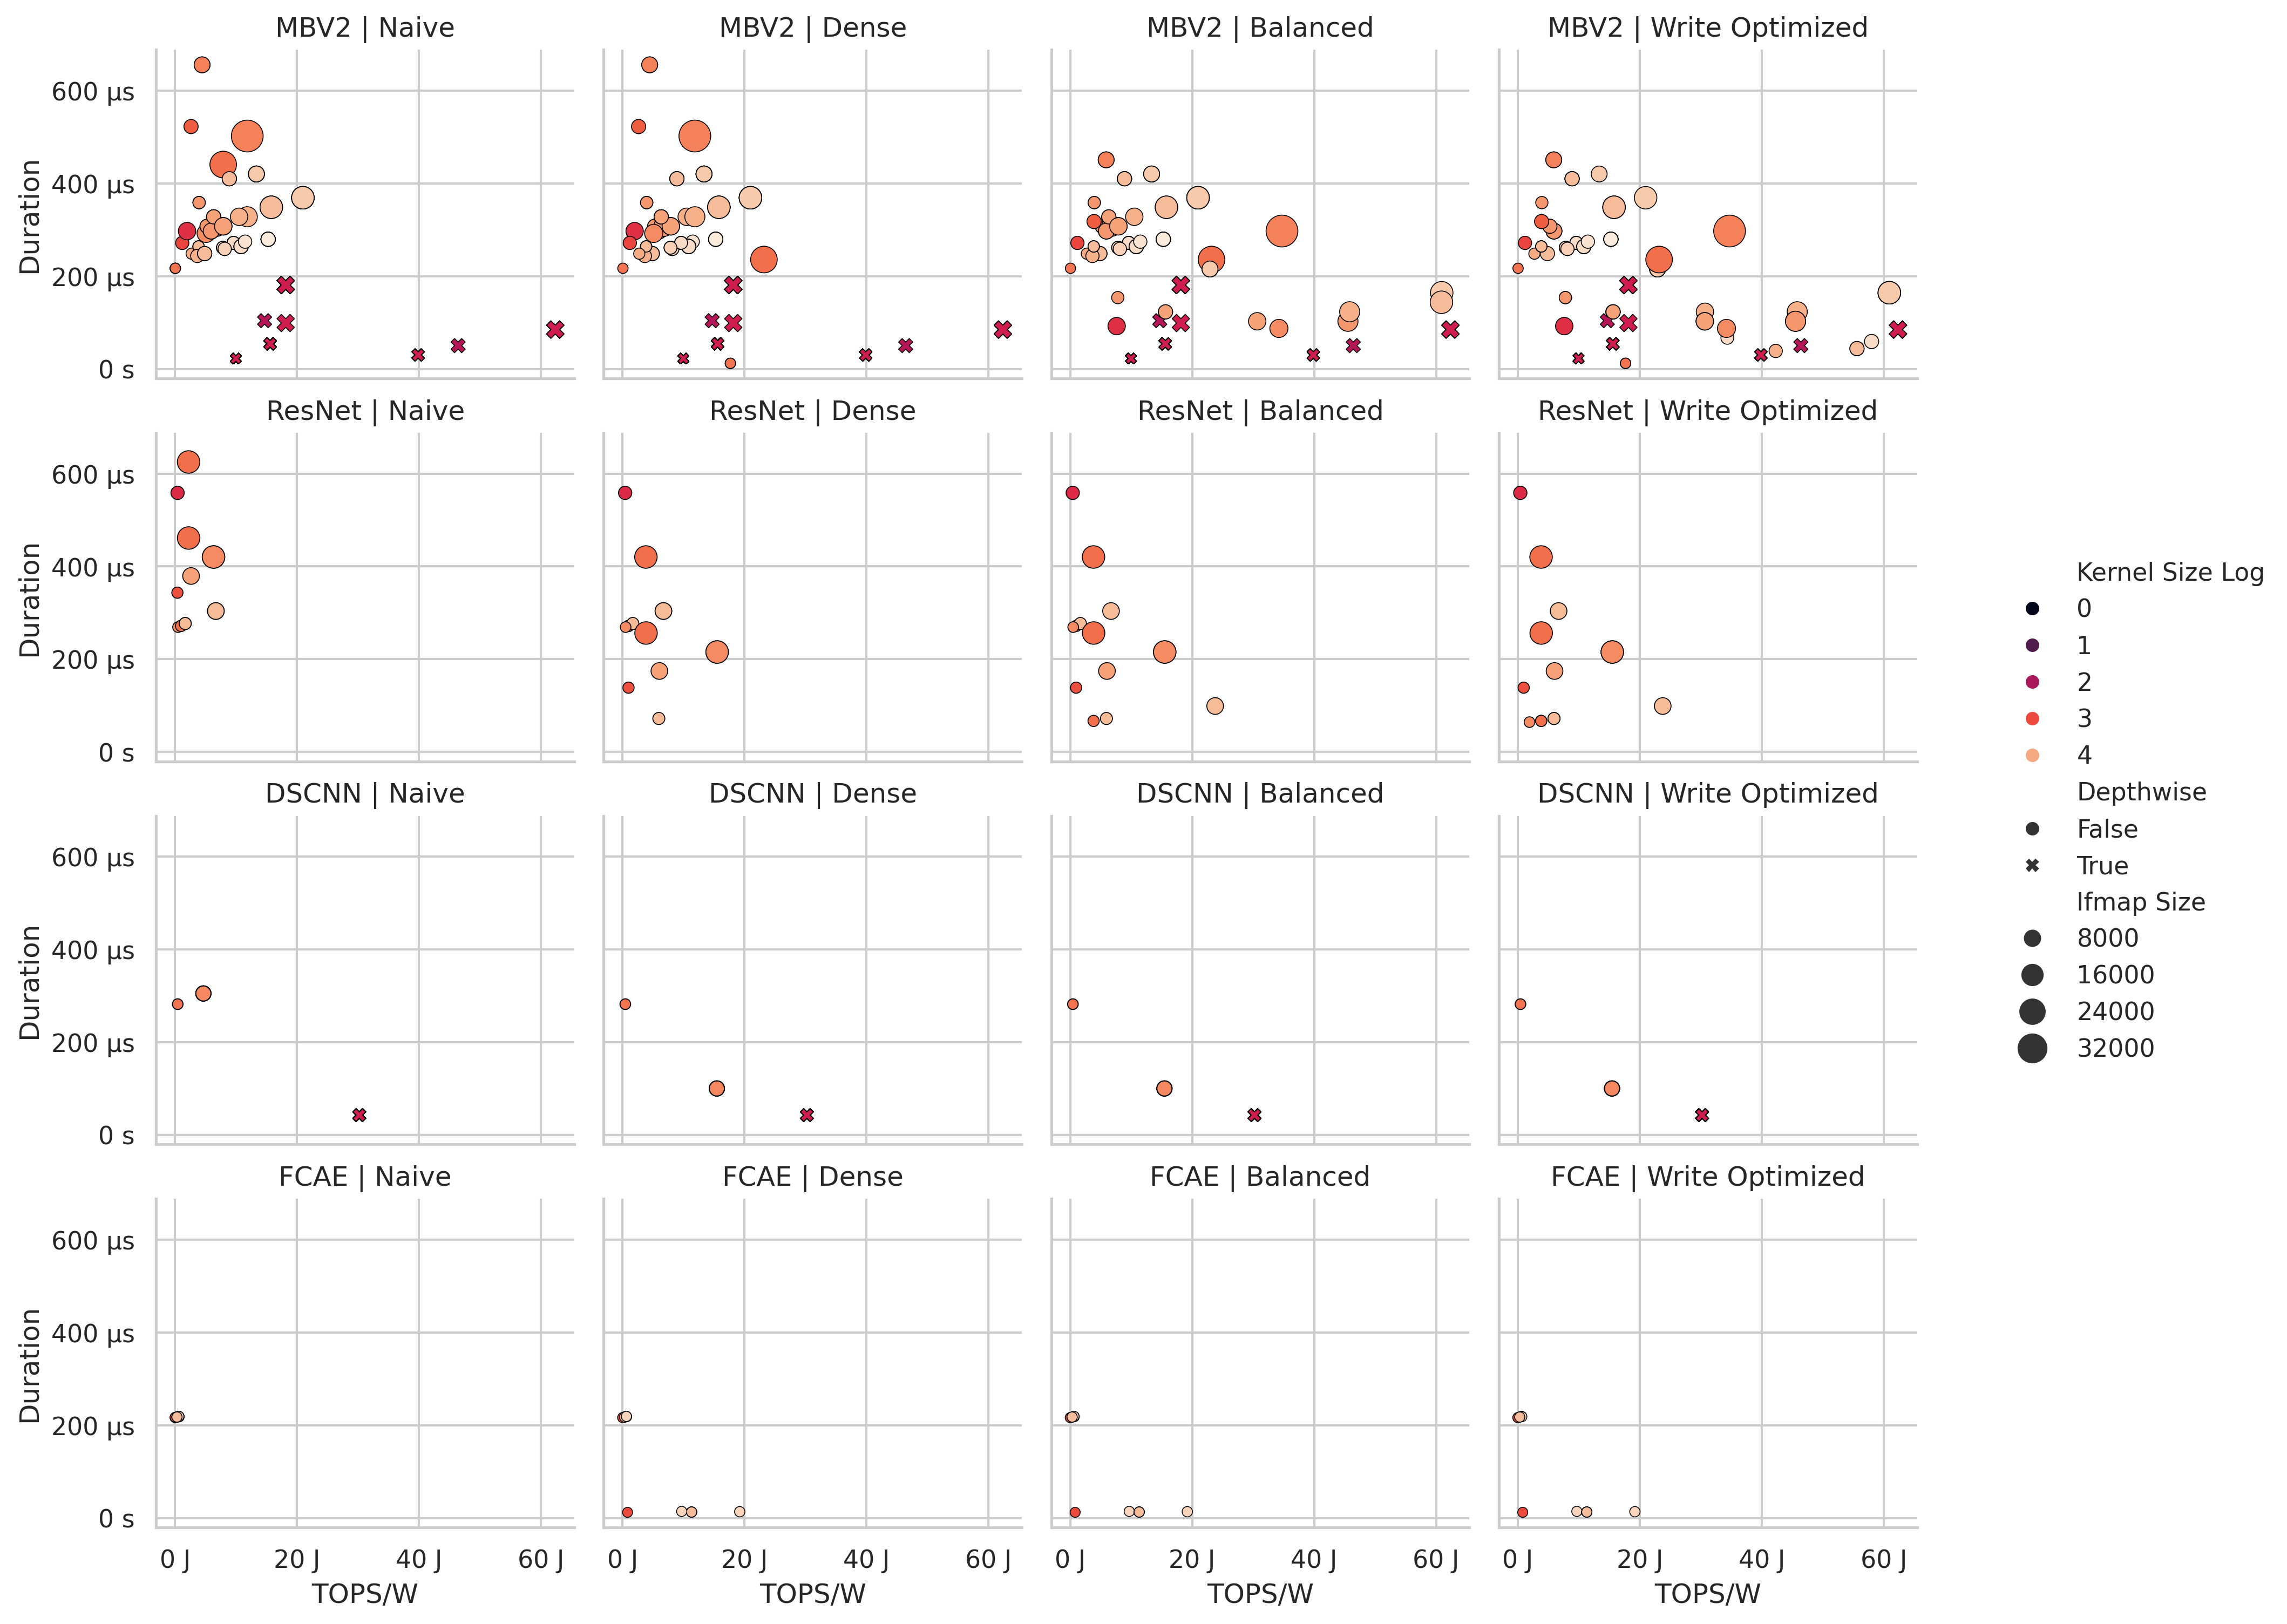
\includegraphics[width=\textwidth]{images/marp_qracc/duration_tops_scatter.png}
    \caption{Scatter plot of the energy vs latency of different layers in the MLPerfTiny models}
    \label{fig:duration_tops_scatter}
\end{figure}

% \section{Hardware Overhead}

% MARP required special hardware (see QRAcc motivations in Chapter \ref{chap:qracc}) to provide the alignment of row inputs and column outputs to the mapped matrix in the AIMC memory array. In terms of the required designs, the feature loader's fundamental design as a register file allows alignment of row inputs to the mapped matrix in the AIMC memory array. Then, an aligner fixes the column output alignment at the end, which is the only datapath overhead of MARP. 

% The feature loader's design, while allowing the row offsets required by MARP, is not easily factored into an "offset-allowing" portion and one that is not. This is because the way we designed the feature loader needs to be able feature loader to be able to load the features in a way that allows for any row offset. Hence, the feature loader is not a MARP-specific design, but rather a design that works well with MARP.

% The output aligner is the only true overhead of MARP. However, we showed in Figure \ref{fig:qracc_area_distribution} that the output aligner only accounts for 1.1\% of the total area of QRAcc. This is a very small overhead compared to the overall area of QRAcc, which is dominated by the SeqAcc memory array and the WSAcc digital core. Furthermore, this area contribution does not even account for the area of the SeqAcc memory array, which is the main component of QRAcc. 

% Hence, the hardware overhead of MARP is minimal and does not significantly impact the overall performance of the QRAcc architecture.

\section{Conclusion}

In this chapter, we presented the results of MARP on QRAcc, our hybrid AIMC accelerator architecture. MARP achieves significant improvements in energy efficiency and inference latency across various MLPerfTiny models, with an average energy consumption reduction of 26.19\% and latency reduction of 19.65\% for MobileNetV2 inference. The statistics extraction method from QRAcc was detailed, alongside the energy and latency results that showcase the advantages of using MARP. The findings indicate that MARP's optimization strategies are effective in enhancing the performance of hybrid AIMC architectures like QRAcc, making them more suitable for edge AI applications.

We'd like to note that we demonstrated MARP with QRAcc in this chapter. However, it can be applied to many other AIMC accelerators. For AIMC accelerators that use multibit non-volatile memories that take a lot of write energy and latency, we believe that MARP will be even better for them. Multibit AIMC memories like PCM and RRAM take a lot of write energy and latency (due to the write-verify method), which MARP can significantly reduce. Furthermore, QRAcc only supports 1b weights at the moment. If QRAcc were to support multibit weights, we would be able to further show reduction as there will be more weights to write.